%-------------------------------------
% This template comes from Anish Athalye (Unofficial University of Cambridge Poster Template). 

% The Poster Template has been modified by Dr. Rahul Raoniar to fulfill B.Tech/Master/Ph.D./PostDoc student's poster presentation requirements.

% Description: I made this unofficial Poster Template for the Indian Institute of Technology Bombay (IITB). Feel free to use it, modify it, and share it. 

% Thank you note: A huge thanks goes to Anish Athalye for the original template.
%-------------------------------------


\documentclass[final,20pt]{beamer}

% ====================
% Packages
% ====================

\usepackage[T1]{fontenc}
\usepackage{lmodern}
\usepackage[orientation=portrait,size=a1,scale=1.2]{beamerposter}
\usetheme{gemini}
\usecolortheme{nott}
\usepackage{graphicx}
\usepackage{booktabs}
\usepackage{tikz}
\usepackage{pgfplots}
\pgfplotsset{compat=1.14}
\usepackage{anyfontsize}
\usepackage{xcolor}
\usepackage{colortbl}
\usepackage[skip=2pt,font=large]{subcaption}
\usepackage{adjustbox}

% ----------------------------------
% For plotting study methodology
% ----------------------------------

\usepackage{tikz}
\usetikzlibrary{shapes.geometric, arrows, arrows.meta, positioning, calc}

% Defining Tickz Style
\tikzstyle{startstop} = [rectangle, rounded corners, minimum width=3cm, minimum height=1cm, text centered, text width = 10cm, draw=black, fill=white]

% \tikzstyle{io} = [trapezium, trapezium left angle=70, trapezium right angle=110, minimum width=3cm, minimum height=1cm, text centered, text width = 4.5cm, draw=black, fill=blue!30]

\tikzstyle{process} = [rectangle, minimum width=3cm, minimum height=1cm, text centered, text width = 6cm, draw=black, fill=white, text width = 10cm]

% \tikzstyle{decision} = [diamond, minimum width=3cm, minimum height=1cm, text centered, draw=black, fill=green!30]

\tikzstyle{arrow} = [ultra thick,->,>=stealth]


% ====================
% Lengths
% ====================

% If you have N columns, choose \sepwidth and \colwidth such that
% (N+1)*\sepwidth + N*\colwidth = \paperwidth
\newlength{\sepwidth}
\newlength{\colwidth}
\setlength{\sepwidth}{0.025\paperwidth}
\setlength{\colwidth}{0.45\paperwidth}

\newcommand{\separatorcolumn}{\begin{column}{\sepwidth}\end{column}}

% ====================
% Title
% ====================

\title{Learning Curve-Informed RL for Efficient Hyperparameter Optimization}

\author{Han-Syuan Liao\inst{1} \and Cheng-An Tsai\inst{1} \and Yi-Xiang Yu\inst{1}}

\institute[shortinst]{\inst{1} Department of Computer Science, National Yang Ming Chiao Tung University}

% ====================
% Footer (optional)
% ====================

% Footer removed per request (leaving out \footercontent removes the footer bar)


% ====================
% Logo (optional)
% ====================

% use this to include logos on the left and/or right side of the header:
\logoleft{
\includegraphics[height=7cm]{logos/NYCU_Logo_C.png}}
%\logoright{
\includegraphics[height=8cm]{logos/NYCU_Logo_B.png}}

% ====================
% Body
% ====================

\begin{document}

\begin{frame}[t]
\begin{columns}[t]
\separatorcolumn

\begin{column}{\colwidth}

% ----------------------------------
% Motivation
% ----------------------------------
  \begin{block}{Motivation: tune like a human expert}
    Hyperparameter optimization (HPO) is costly --- every candidate configuration
    needs a (partial) training run. RL-based HPO such as \textbf{Hyp-RL}
    learns a sequential search policy, but treats each evaluation as a
    \emph{black-box scalar}, throwing away the \textbf{learning curve} produced during training.

    \begin{itemize}
      \item Human experts read the \emph{geometry} of the curve --- is the loss still
            dropping fast, decelerating, or plateauing? --- not just the final number.
      \item These derivative signals have a \emph{task-independent} physical meaning,
            so they are a natural substrate for \textbf{transfer across datasets}.
    \end{itemize}
  \end{block}

% ----------------------------------
% Our idea / objectives
% ----------------------------------
  \begin{alertblock}{Our idea: two cheap augmentations to RL-HPO}
    \begin{itemize}
      \item \textbf{(i) Derivative-informed state.} Append first- \& second-order
            derivatives of the observed learning curve $\big(c'(k),\,c''(k)\big)$
            to the agent's state --- structured signal at \textbf{zero extra evaluation cost}.
      \item \textbf{(ii) Cross-dataset transfer.} Meta-train one shared LSTM policy
            across many datasets so it generalizes to \emph{unseen} tasks without
            restarting from scratch.
    \end{itemize}
    \textbf{Question:} \emph{when} do learning-curve derivatives actually help?
  \end{alertblock}

% ----------------------------------
% Framework
% ----------------------------------
 \begin{block}{Framework: a learning curve-informed RL loop}

    % Learning curve-informed RL loop (redesigned, self-contained)
\begin{figure}
\centering
\begin{adjustbox}{max width=\textwidth, center}
\begin{tikzpicture}[
    font=\large,
    box/.style   = {rectangle, rounded corners=8pt, draw=black, line width=1pt,
                    minimum height=2.8cm, text centered, align=center, fill=white},
    policy/.style= {box, fill=blue!10,   draw=blue!55!black,   line width=1.4pt, minimum width=6.6cm},
    env/.style   = {box, fill=gray!12,   draw=gray!55!black,   line width=1.4pt, minimum width=6.6cm},
    deriv/.style = {box, fill=orange!20, draw=orange!80!black, line width=1.8pt, minimum width=6.6cm},
    state/.style = {box, fill=blue!4,    draw=black,           line width=1.4pt, minimum width=33cm, minimum height=2.8cm},
    fwd/.style   = {-{Stealth[length=6mm,width=5mm]}, line width=1.8pt},
    fb/.style    = {-{Stealth[length=6mm,width=5mm]}, line width=1.8pt, gray!55!black},
    fbo/.style   = {-{Stealth[length=6mm,width=5mm]}, line width=2pt, orange!80!black},
    lab/.style   = {font=\normalsize, fill=white, inner sep=3pt},
]

% ---- state row spanning the top ----
\node[state] (state)
     {\textbf{\large State}\;\;
      $s_t=\big(s_{t-1},\;(\lambda_t,\; r_t,\; \textcolor{orange!75!black}{c'(k;\lambda_t)},\; \textcolor{orange!75!black}{c''(k;\lambda_t)})\big)$
      \;\;$\oplus$\;\; static feature $d$};

% ---- middle action row ----
\node[env]    (env)  [below=4.4cm of state] {\textbf{Environment}\\[3pt]{\normalsize train config $\to$ log curve}};
\node[policy] (pi)   [left=7.5cm of env]    {\textbf{Policy} $\pi_\theta$\\[3pt]{\normalsize shared LSTM}};
\node[deriv]  (der)  [right=7.5cm of env]   {\textbf{Derivative}\\\textbf{Extractor}};

% ---- forward flow (left -> right) ----
\draw[fwd] (pi)  -- node[lab,above]{config $\lambda_{t+1}$} (env);
\draw[fwd] (env) -- node[lab,above]{curve $c(k)$}           (der);

% ---- feedback to state (vertical) ----
% policy reads the state (down)
\draw[fb]  (state.south -| pi.north) -- node[lab,left]{read} (pi.north);
% environment returns the reward (up)
\draw[fb]  (env.north) -- node[lab,left]{reward $r_{t+1}$}   (env.north |- state.south);
% derivative features close the loop (up) -- highlighted contribution path
\draw[fbo] (der.north) -- node[lab,right,text=orange!80!black]{\textbf{$c',c''$ features}} (der.north |- state.south);

% ---- legend tag for the contribution ----
\node[font=\normalsize, text=orange!80!black, anchor=west] at ($(der.south)+(-3.3cm,-1.0cm)$)
     {\textbf{$\Leftarrow$ our addition (zero extra cost)}};

\end{tikzpicture}
\end{adjustbox}
\caption{\textbf{Learning curve-informed RL loop.} The policy reads the state and picks
a configuration $\lambda_{t+1}$; the environment trains it and logs the learning curve
$c(k)$; the \textcolor{orange!80!black}{\textbf{Derivative Extractor}} turns that curve
into first/second-order features $c',c''$ appended to the next state --- structured
signal at \emph{zero extra evaluation cost}.}
\label{fig:framework}
\end{figure}


    \heading{State $\to$ Policy $\to$ Environment $\to$ Derivative Extractor $\to$ State}
    We formulate HPO as an MDP: action $=$ choosing a configuration $\lambda$,
    reward $=$ negative generalization error $R(D,a)=-f(D,\lambda{=}a)$. An LSTM
    $Q$-network, primed by a 16-d dataset descriptor $d$, scores configurations.
    Each curve is summarized by \textbf{5 finite-difference features} (final value,
    min, slope, curvature, total improvement) over its last 8 epochs.
    The curve-free ablation is \texttt{HyperRL}; the full method is \texttt{LC-DQN}.

    \begin{figure}
      \centering
      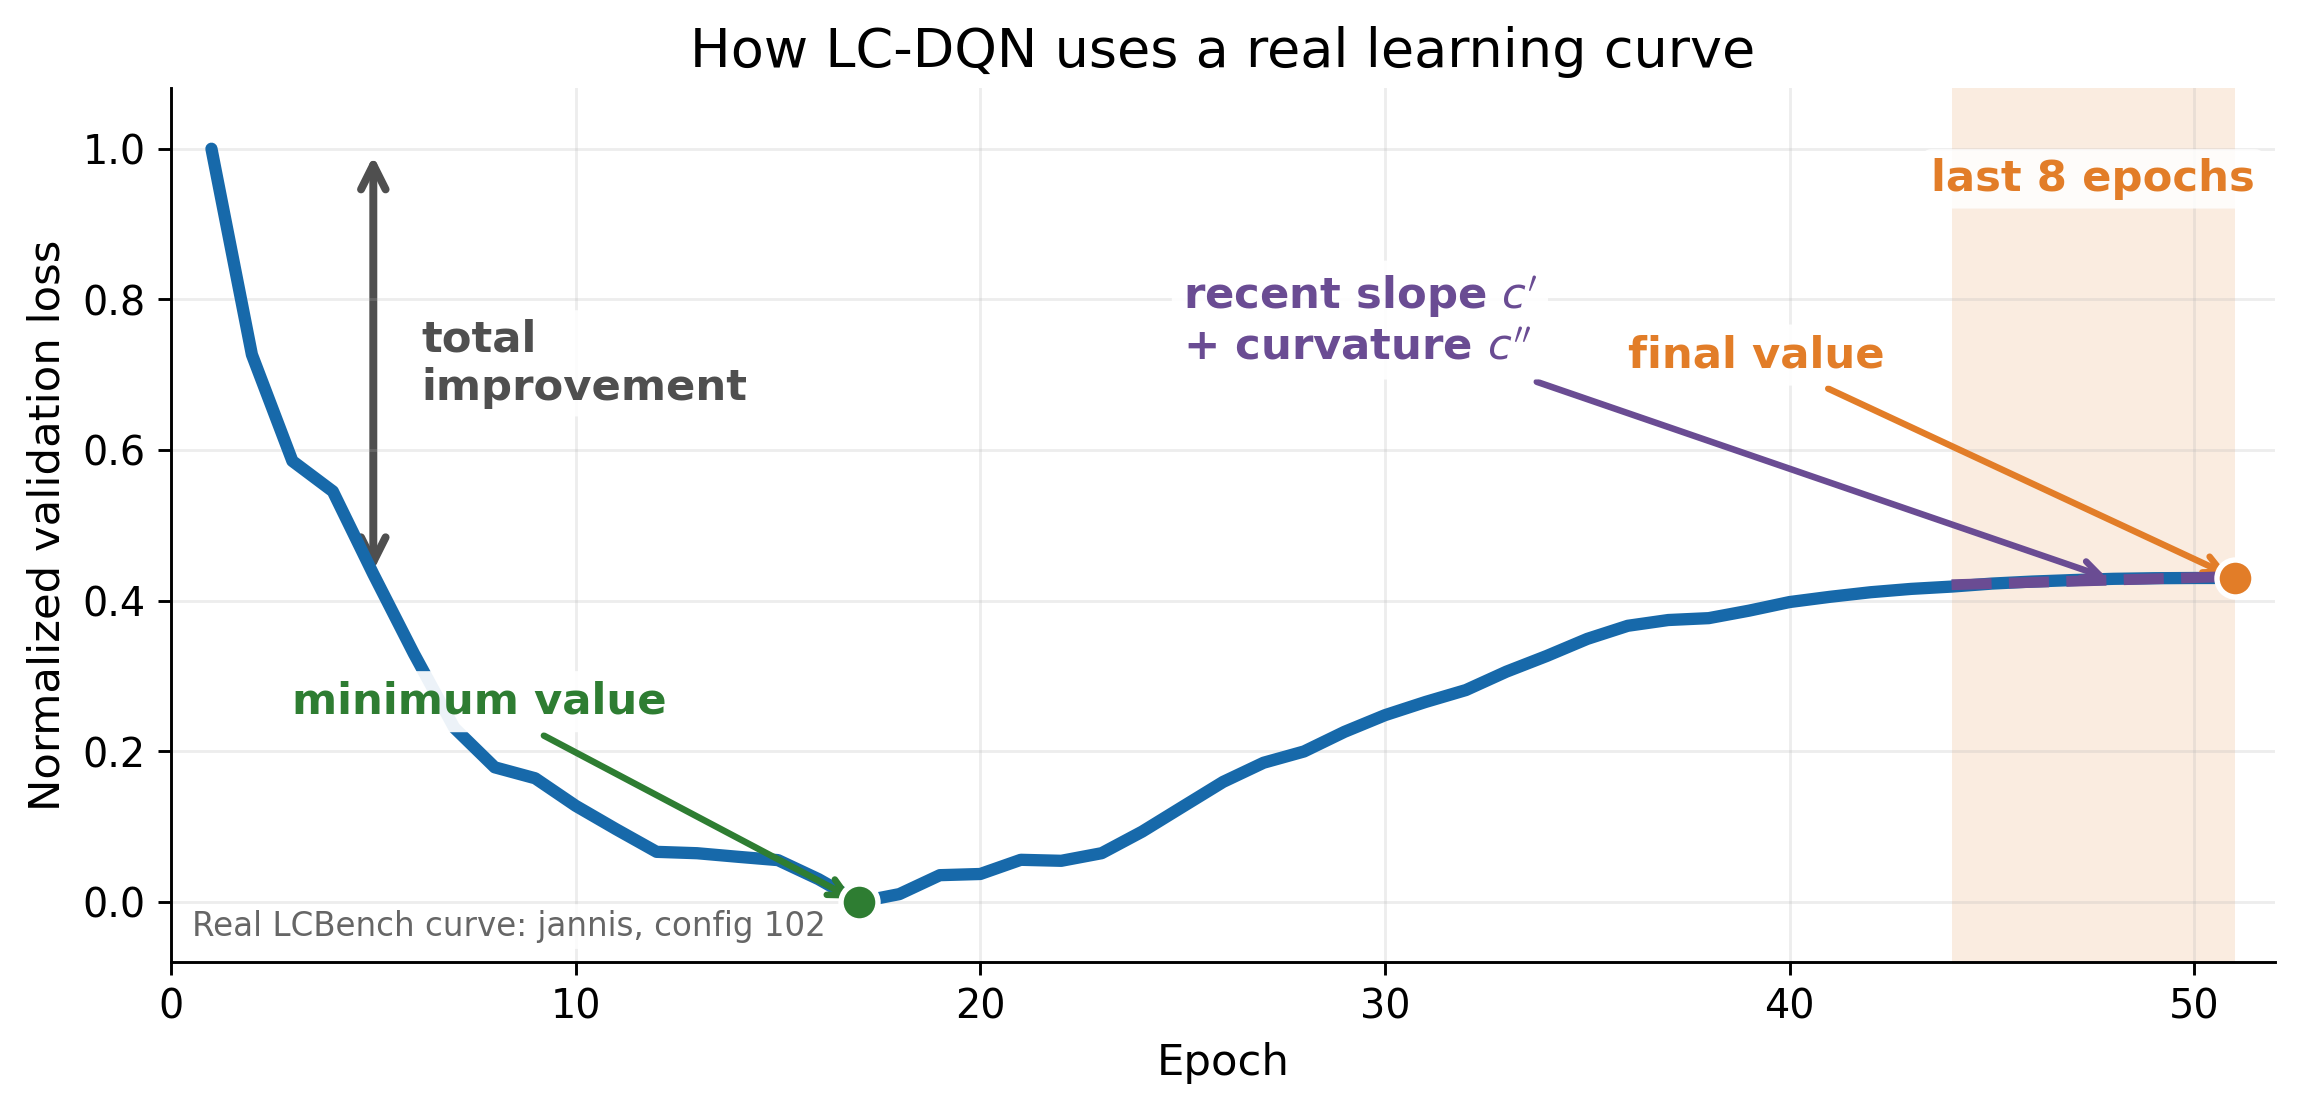
\includegraphics[width=0.92\textwidth]{images/learning_curve_features.png}
    \end{figure}
 \end{block}

% ----------------------------------
% Setup
% ----------------------------------
\begin{block}{Experimental setup}
    \begin{itemize}
      \item \textbf{LCBench}: 35 \emph{homogeneous}
            OpenML tasks --- same MLP family, 7-d search space, 50-epoch protocol
            $\Rightarrow$ stereotyped, near-monotone curves.
      \item \textbf{Kaggle Playground Series}: 15 \emph{heterogeneous} tabular tasks
            (regression \& classification), diverse curve shapes $\Rightarrow$
            the regime transfer is hard.
      \item Baselines: Random Search, Bayesian Optimization
            (Gaussian-process surrogate). Meta-policies
            frozen after training; evaluation budget $=20$.
    \end{itemize}
\end{block}

\end{column}

\separatorcolumn

\begin{column}{\colwidth}

% -------------------------------
% Key result
% -------------------------------
\begin{block}{Key result: the same agent, two regimes}

    \textbf{Identical agent and ablation} (\texttt{LC-DQN} vs.\ curve-free
    \texttt{HyperRL}) on a homogeneous and a heterogeneous benchmark --- the curve
    features help \emph{only} when curve shapes vary.

    \begin{figure}
      \centering
      \begin{subfigure}{0.55\textwidth}
        \centering
        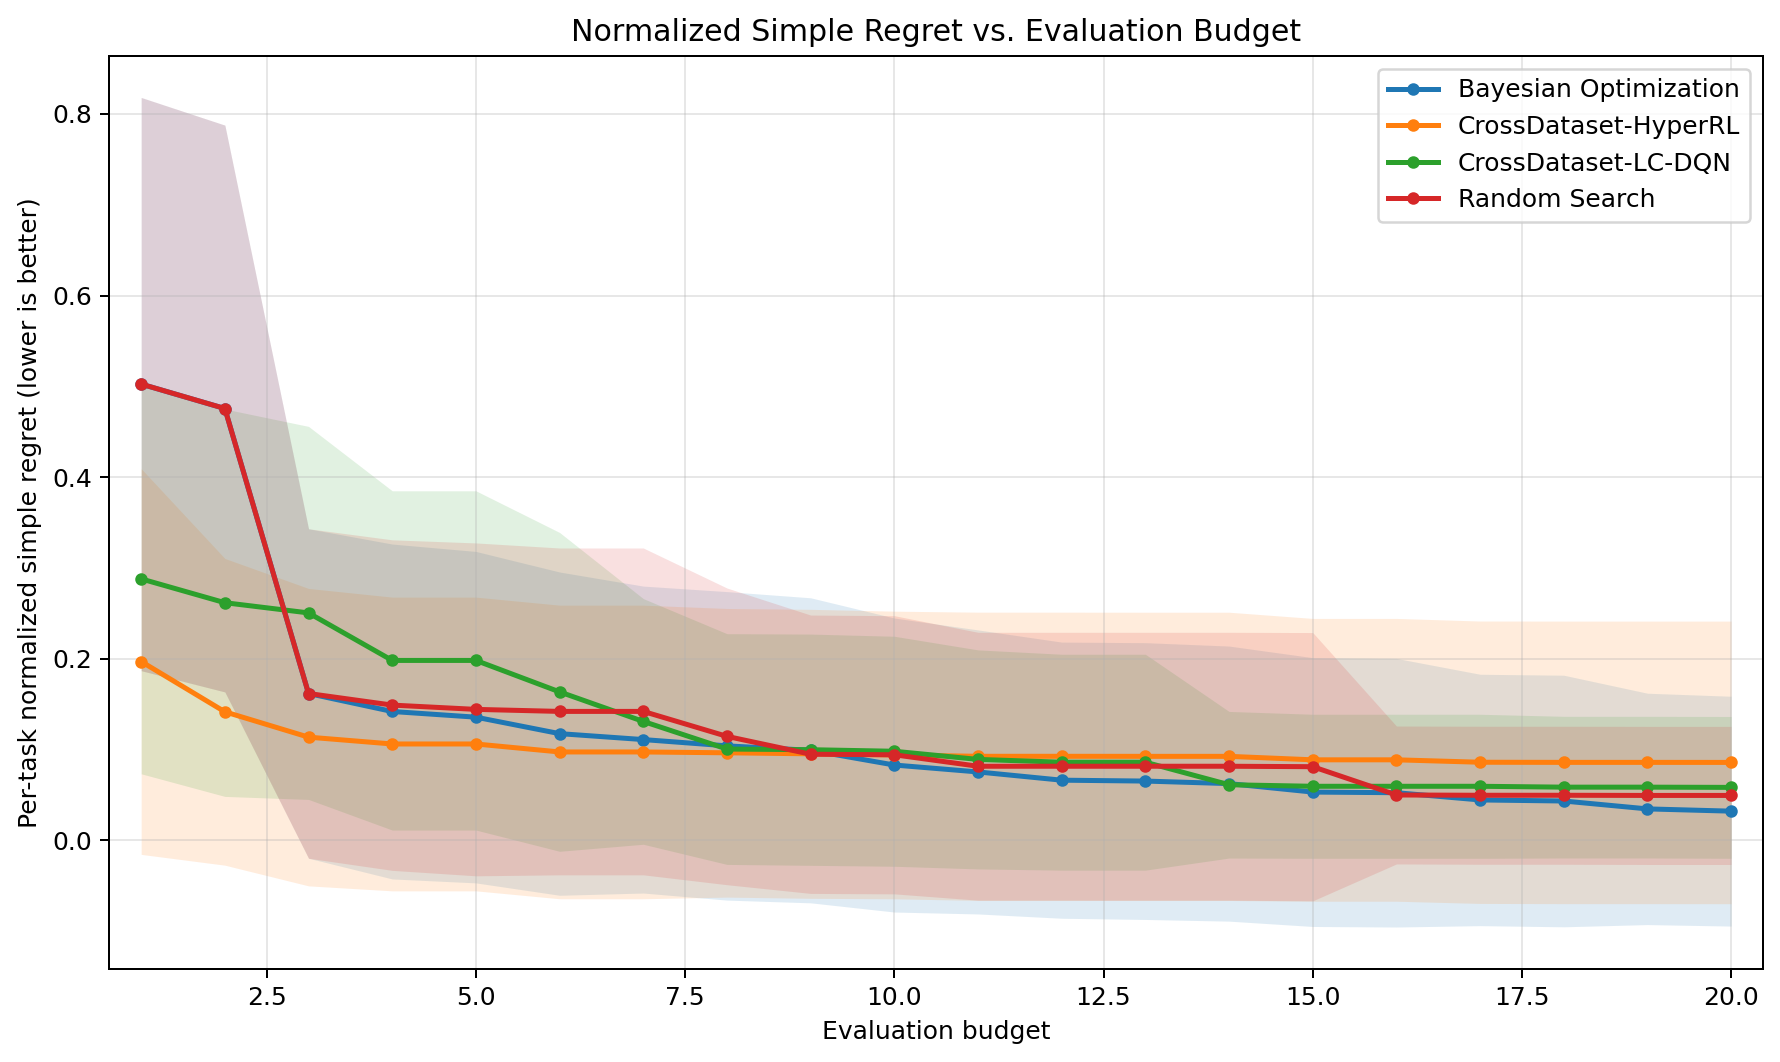
\includegraphics[width=\textwidth]{images/20_budget.png}
        \caption{\textbf{LCBench (homogeneous):} \texttt{LC-DQN} (green) $\approx$
        \texttt{HyperRL} (orange) --- \emph{no gain}.}
      \end{subfigure}

      \vspace{0.6em}

      \begin{subfigure}{0.55\textwidth}
        \centering
        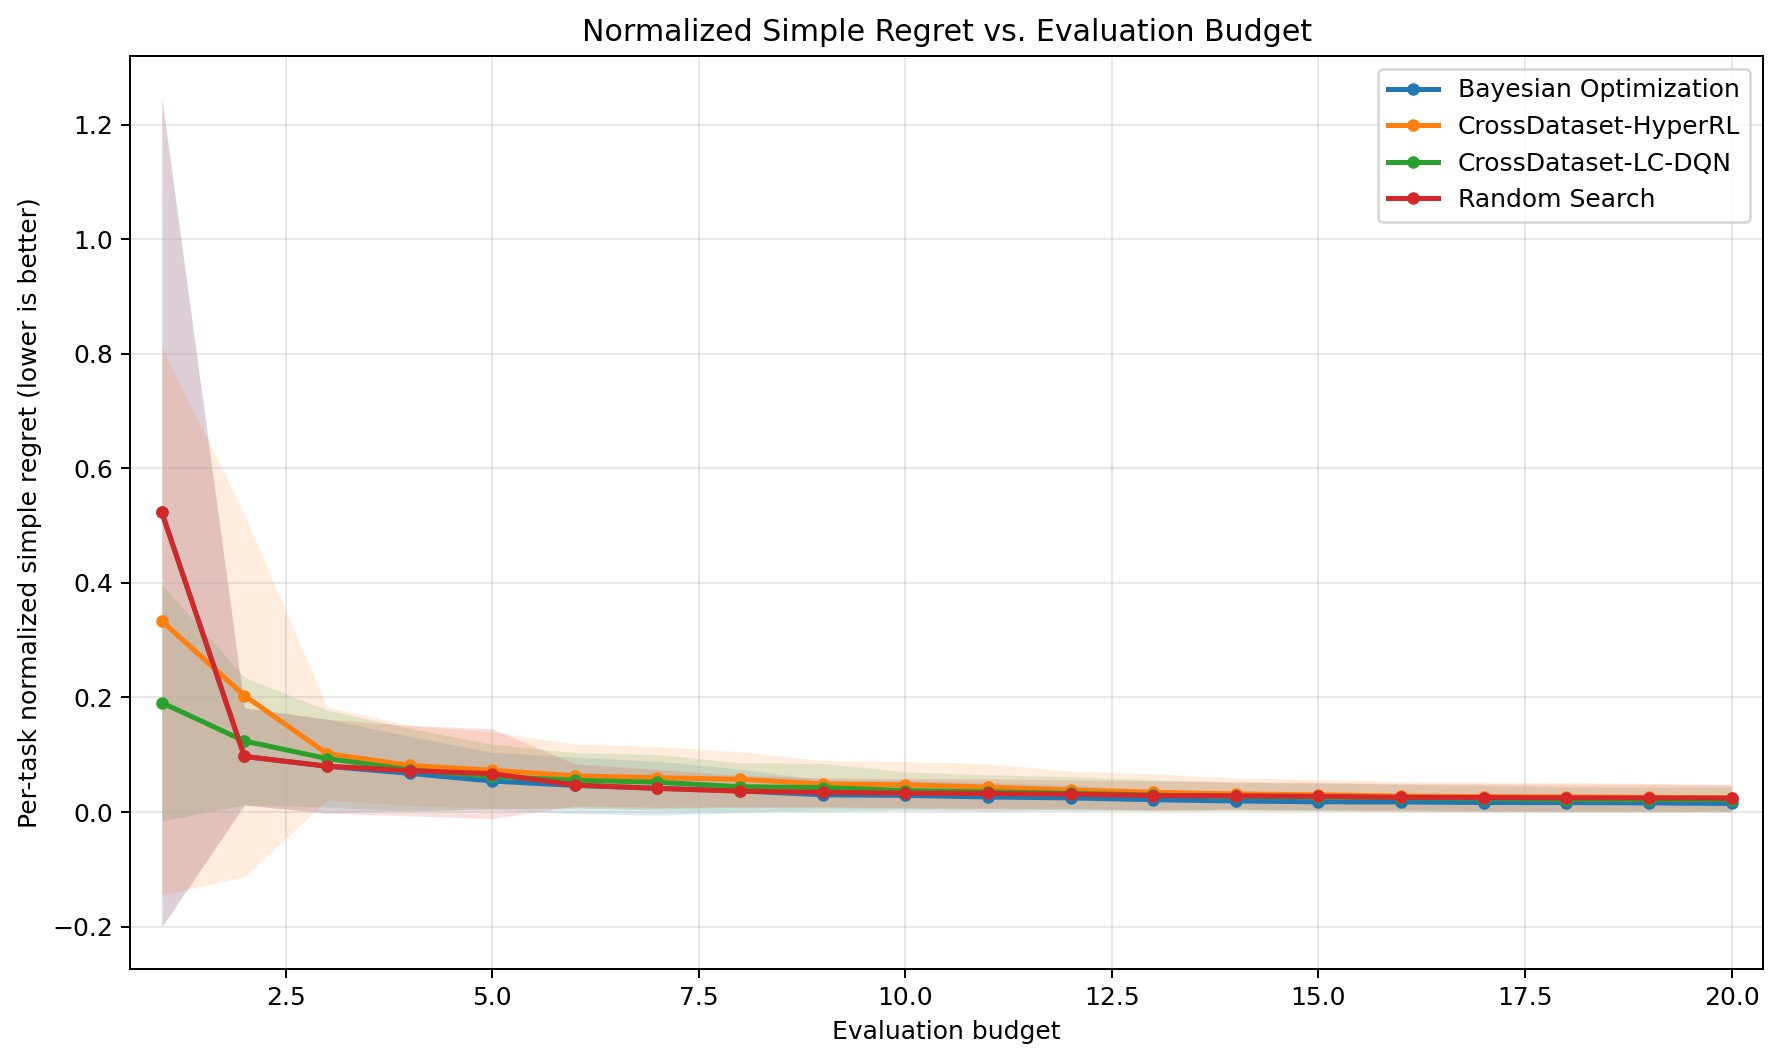
\includegraphics[width=\textwidth]{images/kaggle_eval_budget.png}
        \caption{\textbf{Kaggle (heterogeneous):} \texttt{LC-DQN} (green) clearly
        below \texttt{HyperRL} (orange) --- \emph{consistent cold-start gain}.}
      \end{subfigure}
      \caption{Normalized simple regret vs.\ evaluation budget (lower is better);
      same two RL variants on both benchmarks.}
    \end{figure}

    \begin{table}
  \centering
  \caption{Average normalized simple regret on the 15 heterogeneous Kaggle
  Playground tasks (5 seeds; lower is better). The curve features are what push
  the RL agent below Random Search.}
  \begin{tabular}{l c c}
    \toprule
    \textbf{Method} & \textbf{Norm.\ regret} $\downarrow$ & \textbf{Avg.\ rank} \\
    \midrule
    Bayesian Opt.\ (GP, asymptotic best)    & 0.0150 & --- \\
    \rowcolor{orange!18}
    \textbf{LC-DQN} (ours, +curve features) & \textbf{0.0217} & \textbf{2.33} \\
    Random Search                           & 0.0243 & --- \\
    HyperRL (curve-free ablation)           & 0.0251 & 2.87 \\
    \bottomrule
  \end{tabular}
  \label{tab:results}
\end{table}


    The two variants differ \emph{only} in the appended derivative features, so the
    Kaggle gap ($0.0217$ vs.\ $0.0251$) is directly attributable to the
    learning-curve signal --- transfer alone does not beat Random Search.
\end{block}

% -------------------------------
% Conclusion / key takeaway (merged insight + conclusions)
% -------------------------------
   \begin{alertblock}{Conclusion: derivatives help when curve \emph{shape} varies}
    \begin{itemize}
      \item \textbf{LCBench (homogeneous):} \texttt{LC-DQN} $\approx$ \texttt{HyperRL} ---
            smooth, monotone curves are already well-predicted by the static descriptor
            + scalar reward, so derivatives add little.
      \item \textbf{Kaggle (heterogeneous):} diverse curve geometries (steady improvers,
            early plateaus, overfitters) --- derivatives supply discriminative cold-start
            signal, the \emph{only} RL variant to beat Random Search.
      \item \textbf{Cheap \& zero-cost:} the derivative features are appended for free and
            pay off precisely when curve \emph{shape} varies across configurations.
      \item \textbf{Transfer + asymptotics:} the frozen cross-dataset policies start strong
            (transfer pays off at cold-start); Bayesian Optimization still wins asymptotically ($0.0150$).
    \end{itemize}
  \end{alertblock}

% -------------------------------
% Future work
% -------------------------------
  \begin{exampleblock}{Future work}
    \textbf{Surrogate-accelerated evaluation:} replace full training runs with a
    multi-dataset surrogate, letting the agent exploit the curve signal across far
    more datasets at a fraction of the cost.
  \end{exampleblock}

\end{column}
\separatorcolumn

\end{columns}
\end{frame}

\end{document}
